\section{实践}
\subsection{论文排版}


\subsection{论文模板使用}
\begin{frame}[fragile]
  \frametitle{模板}
  \begin{itemize}
    \item<+-> 是什么?
  
      \begin{itemize}
        \item 设计好的格式框架
        \item 专注于内容:\alert{不要追求与期刊排版一致}
        \item Word 中的样式:「学好 \LaTeX{} 可以更科学地使用 Word」
      \end{itemize}
  
    \item<+-> 有哪些?
  
      \begin{itemize}
        \item 期刊:\pkg{revtex}、\pkg{elsarticle}、\pkg{IEEEtran}、\pkg{acmart}……
        \item 学位论文:\pkg{thuthesis}、\pkg{ustcthesis}、\alert{\pkg{sustechthesis}}……
      \end{itemize}
  
    \item<+-> 怎么用?
  
      \begin{itemize}
        \item |\documentclass{...}|,配置参数,照常编写
        \item \alert{看文档,看文档,看文档}
      \end{itemize}
  
    \item<+-> 去哪里找?
  
      \begin{itemize}
        \item CTAN \link{https://ctan.org} 或 GitHub \href{https://github.com}{\faGithub}
        \item 期刊官网
        \item 「U 盘拷给你的模板一定是过时的」
      \end{itemize}
  \end{itemize}
\end{frame}


\begin{frame}{论文排版}
    \begin{itemize}
      \item 获取模板
        \begin{itemize}
          \item 随发行版自带、手动官网下载
          \item 模板文档类 \texttt{.cls} 文件
          \item 示例 \texttt{.tex} 文件
        \end{itemize}
      \item 编辑 \texttt{.tex} 文件:添加用户内容
      \item 编译:生成 PDF 文档
    \end{itemize}
  \end{frame}
  
  % \begin{frame}[fragile]{论文排版举例}
  %   \begin{exampleblock}{IEEE 期刊论文}
  %     \begin{itemize}
  %       \item 获取模板:已随发行版自带
  %         \begin{itemize}
  %           \item 在安装目录 |<prefix>\texlive\2020\texmf-dist\doc\latex\IEEEtran|
  %             下找到 |bare_jrnl.tex|
  %           \item 复制到某个文件夹(比如个人存论文的目录)
  %         \end{itemize}
  %       \item 编辑 |bare_jrnl.tex| 文件 (英文模板:不支持中文)
  %       \item 编译
  %         \begin{itemize}
  %           \item 英文文献:\XeLaTeX 、\pdfLaTeX 编译均可
  %         \end{itemize}
  %     \end{itemize}
  %   \end{exampleblock}
  % \end{frame}



\subsection{常用模板}
\begin{frame}{在作业中常用的模版}
    \begin{columns}[c]
    \begin{column}{.45\textwidth}
        \begin{itemize}
            \item math201实验报告模板 \link{https://github.com/SUEPaper/math201-latex-report}
            \item 上海电力大学学位论文模板SUEPThesis(目前还在开发中。。。) \link{https://github.com/SUEPaper/SUEPThesis}
        \end{itemize}
    \end{column}
    \begin{column}{.45\textwidth}
        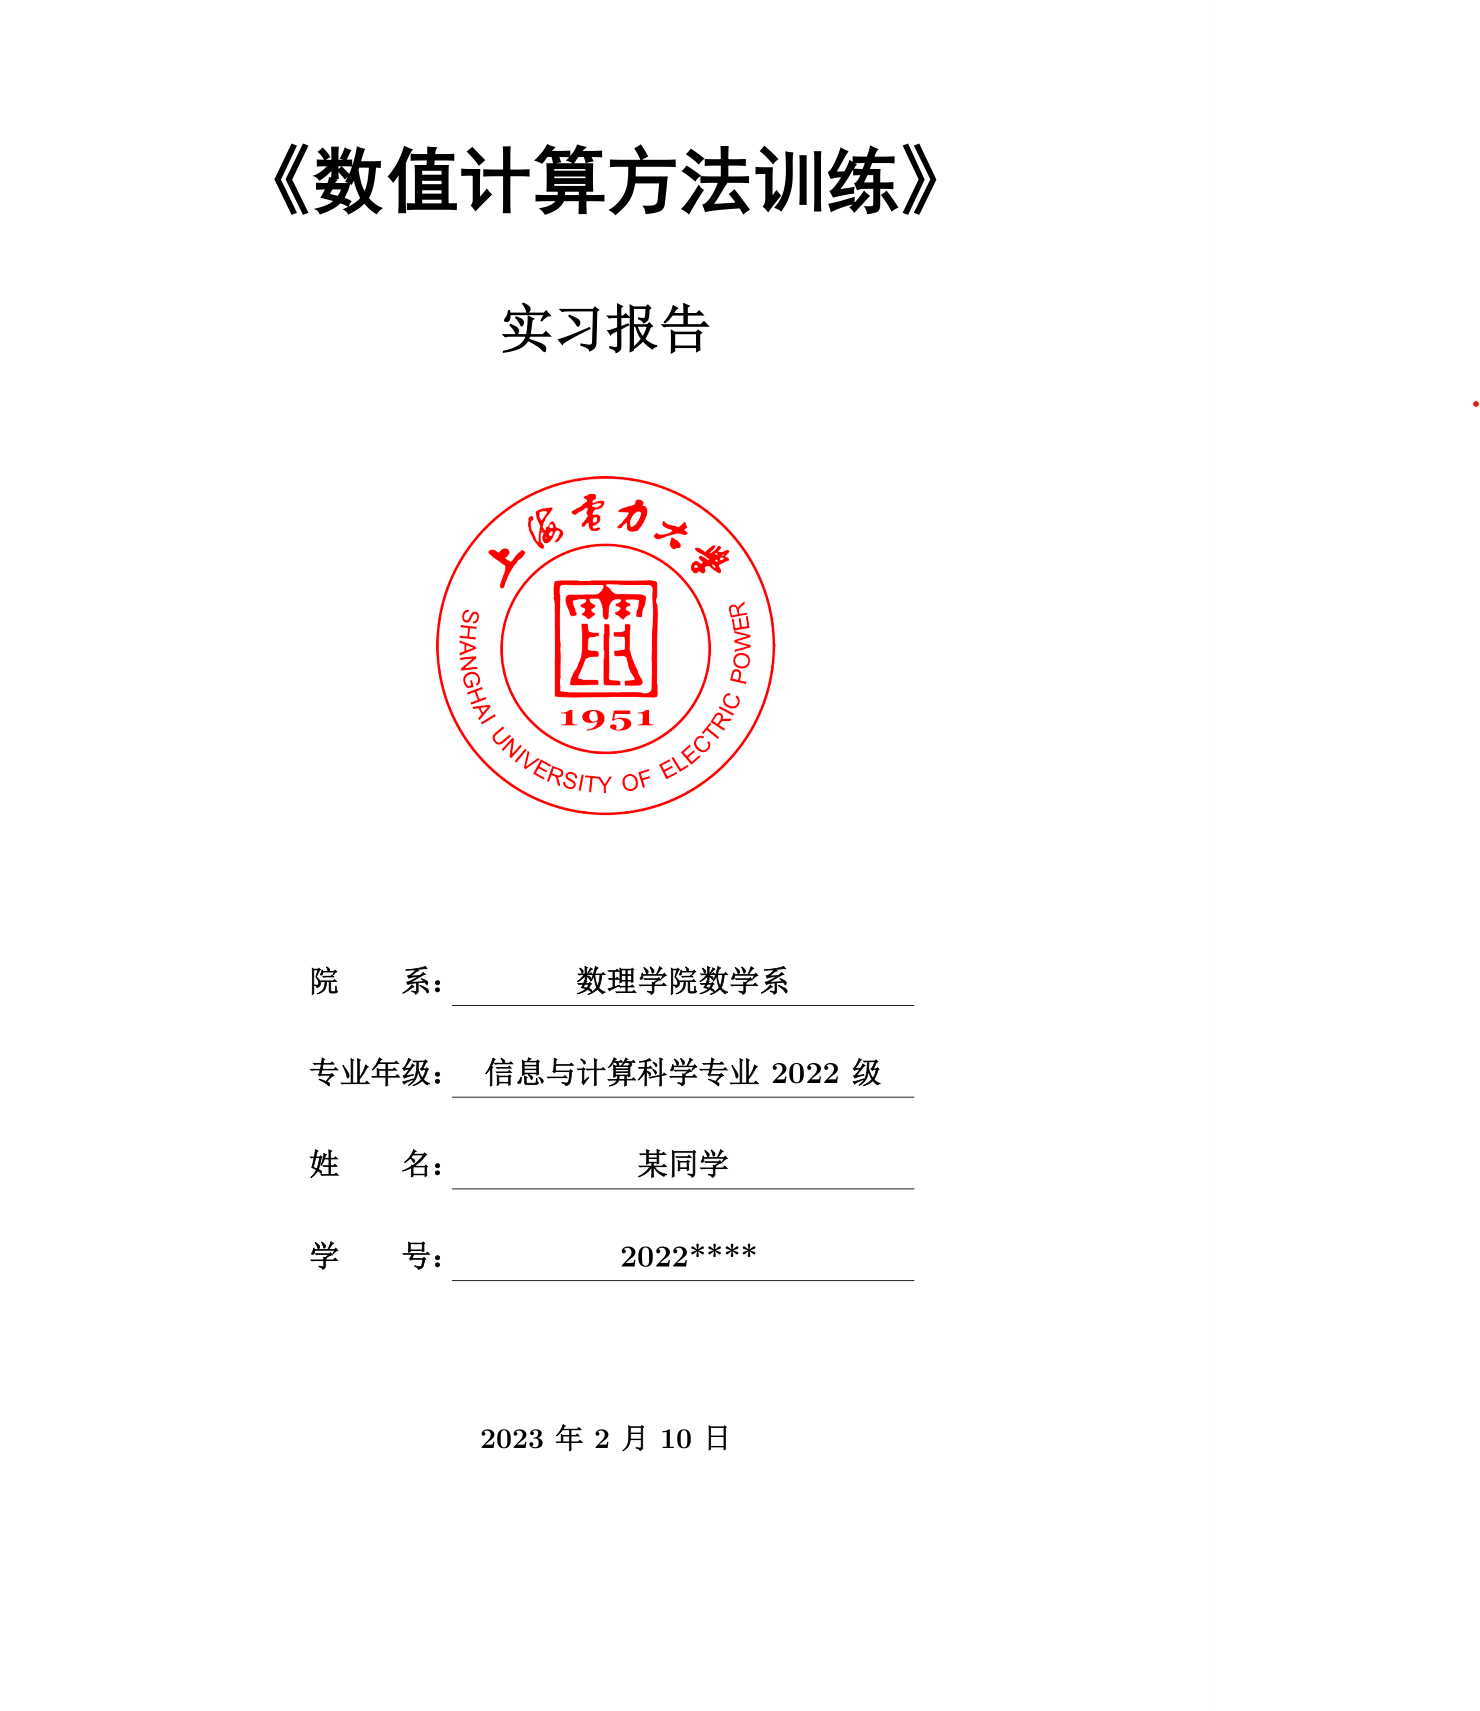
\includegraphics[width=0.75\textwidth]{examples/math201.png}
      \end{column}
    \end{columns}
\end{frame}
